\chapter{Resultados Obtenidos y Análisis}
A continuación se presentan los resultados de los 4 experimentos realizados. El orden de presentación será de la siguiente forma: (i) resultados para el caso Høvsore sin DA, es decir, la validación de la metodología, (ii) caso Høvsøre con DA puntual, (iii) caso Bolund sin DA y (iv) caso Bolund con DA multipunto. Todos los resultados son obtenidos de la malla mas interior para cada dominio, es decir, d07 para Høvsore y d08 para Bolund. El cálculo de los espectros espaciales está hecho en base a: (a) valores obtenidos para un nivel $\eta$ en particular, (b) promedios temporales sobre las ventanas de tiempo válidas de simulación y sobre cada número de onda asociado a la discretización de la malla, y (c) un promedio móvil para eliminar ruido del espectro.
\section{Caso I: Høvsøre}
Tomando en consideración que los resultados para este caso son válidos desde las 12:00 hasta las 18:00 del día simulado, se busca a través de esta sección evidenciar cuatro aspectos relevantes del modelo: (i) La respuesta del modelo LES al escalamiento dinámico y la alta resolución, (ii) la concordancia entre los datos simulados y aquellos obtenidos por Peña en el año 2013, (ii) la concordancia entre los datos simulados y la serie de tiempo medida en el mástil meteorológico y (iv) la concordancia de las variables de segundo orden con aquellas canónicas para flujo en terreno plano homogéneo.

\subsubsection{Estratificación y Largo de Capa Límite}
En primer lugar se revisa la estabilidad del flujo para la ventana de tiempo seleccionada. Tomando en cuenta que según la literatura este debería ser un caso de atmósfera neutra, la Figura \ref{fig:06_hov_pbl} muestra la evolución del perfil de temperatura potencial virtual a través de toda la simulación para el punto de control en el mástil meteorológico. Debido a la homogeneidad del terreno, los perfiles de temperatura potencial virtual en el resto del dominio son, a grandes rasgos, idénticos, y por lo tanto se puede hablar que el perfil mostrado es representativo de todo el dominio. En este se puede notar como la estratificación del campo va cambiando a medida que avanza en el ciclo diurno la simulación, desde una atmósfera inestable en la mañana, hasta la estabilidad en la noche. Notar que, tal cual como expuso Peña, se tiene un perfil estable desde las 12:00 hasta las 15:00 horas, ventana de tiempo que cae dentro de los resultados válidos del modelo y por ende, será en esta ventana en la cual se extraerán resultados.

\begin{figure}[H]
	\begin{minipage}{0.5\linewidth}
		\centering{\hspace{0.9cm}(a)}
	\end{minipage}%
	\begin{minipage}{0.5\linewidth}
		\centering{\hspace{0.6cm}(b)}
	\end{minipage}%
	
	\begin{minipage}{0.5\linewidth}
		\centering
		\includegraphics[width=0.86\linewidth,trim={0cm 5mm 0cm 0mm},clip]{Imagenes/06/hov/pbl}%
	\end{minipage}%
	\begin{minipage}{0.5\linewidth}
		\centering
		\includegraphics[width=0.86\linewidth,trim={0cm 5mm 0cm 0cm},clip]{Imagenes/06/hov/temp_profile}%
	\end{minipage}%
	
	\caption{Ciclo diurno-nocturno del perfil de temperatura potencial en el mástil meteorológico. (a) Resultados cada 20 minutos del perfil de $\theta_v$. (b) Corresponde al detalle del perfil dentro de la capa límite atmosférica ($\delta \approx 750$ [m]).}
	\label{fig:06_hov_pbl}
\end{figure}

A través de la misma Figura \ref{fig:06_hov_pbl} es posible estimar el \textbf{alto de la capa límite} como el punto en altura justo antes de la inversión térmica. Utilizando este acercamiento es fácil notar como el espesor de ABL varía durante el día desde un valor cercano a los 800 [m] hasta unos 400 [m] en la noche. Se decide utilizar un valor promedio de $\delta = 750$ [m] para adimensionalizar los resultados futuros.
\subsubsection{Estructuras del Campo de Velocidades}
Con respecto a las variables de primer orden y el rendimiento del LES, la Figura \ref{fig:06_hov_eta1} muestra los campos instantáneos de velocidad para el primer nivel vertical $z_1\approx 5.25$ [m] del dominio más interior d07 a las 15:00\footnote{Si bien la selección de la hora es arbitraria, cualquier hora después de las 12:00 hubiese servido y de hecho el comportamiento del campo no varía mucho.}. Acá se pueden apreciar de manera visual las estructuras que genera el LES sobre el campo de velocidades. 
\begin{figure}[H]
	\centering
	\begin{minipage}{0.5\linewidth}
		\center\hspace{0.3cm}(a)
	\end{minipage}%
	\begin{minipage}{0.5\linewidth}
		\center\hspace{0.3cm}(b)
	\end{minipage}%
	
	\includegraphics[width=0.5\linewidth,page=55,trim={2.5cm 6.2cm 1cm 4.5cm},clip]{Imagenes/06/hov/eta1_u}%
	\includegraphics[width=0.5\linewidth,page=55,trim={2.5cm 6.2cm 1cm 4.5cm},clip]{Imagenes/06/hov/eta1_v}%
	
	\center{\hspace{0.3cm}(c)}
	
	\includegraphics[width=0.5\linewidth,page=55,trim={2.5cm 6.2cm 1cm 4.5cm},clip]{Imagenes/06/hov/eta1_V}%
	\caption{(a) Componente $u$ de la velocidad en el primer nivel de la coordenada vertical ($z_1=5.25$ [m]) para las 15:00. (b) Idéntico al anterior pero para la componente $v$. (c) Magnitud del campo de velocidad.}
	\label{fig:06_hov_eta1}
\end{figure}
A una primera vista, se puede concluir que el LES fue aplicado correctamente en el dominio, presentando las estructuras clásicas que se deberían manifestar en el campo de velocidades. En particular, para este caso se puede ver que los contornos de velocidad tienen cierto estiramiento desviándose del comportamiento clásico homogéneo. Esto se explica debido a la dirección preferente que tiene el viento al venir del este (viento a $105^\circ$). La baja de velocidad local que se genera en la esquina inferior derecha se explica debido a la depresión topográfica local que existe en esa zona.
\subsubsection{Comparación de Series de Tiempo}
Para evaluar la calidad del modelo, se muestra la serie de tiempo de los datos simulados junto a lo datos medidos en el mástil meteorológico para la fecha de interés en la Figura \ref{fig:06_hov_ts}. 

\begin{figure}[H]
	\centering
	\includegraphics[width=1\linewidth,trim={9mm 63mm 10mm 55mm},clip]{Imagenes/06/hov/ts_v}%
	
	\includegraphics[width=1\linewidth,trim={12mm 55mm 10mm 55mm},clip]{Imagenes/06/hov/ts_o}%
	\caption{Serie de tiempo para la rapidez instantánea del viento $V$ y su dirección en la ubicación del mástil meteorológico. La línea continua corresponde a lo datos simulados interpolados a las alturas de medición (solo para $V$) y la línea punteada a los datos medidos en el mástil.}
	\label{fig:06_hov_ts}
\end{figure}

En esta Figura, la linea segmentada vertical indica el límite del tiempo de \emph{spinup} y por lo tanto sólo los resultados desde ese punto son válidos. Se puede apreciar que la simulación (en línea continua) capta de buena forma la tendencia de la magnitud de la velocidad para el mástil, sin embargo, la simulación fue incapaz de representar las ráfagas que ocurrieron en esa fecha y que aceleraron al fluido. Un especial déficit de momemtum se lleva a cabo en los niveles superficiales, dando a entender que quizás el modelo de suelo, el modelo de superficie o de turbulencia está actuando de manera muy disipativa en esos niveles. Con respecto a la dirección del viento, esta quedó a grandes rasgos bien representada por la simulación.

\begin{figure}[H]
	\begin{minipage}{0.33\linewidth}
		\centering \hspace{1.5cm}(a)
	\end{minipage}%
	\begin{minipage}{0.33\linewidth}
		\centering \hspace{1cm}(b)
	\end{minipage}%
	\begin{minipage}{0.33\linewidth}
		\centering \hspace{1cm}(c)
	\end{minipage}%
	\vspace{-3mm}
	\begin{center}
	\includegraphics[height=0.62\linewidth,page=37,trim={35mm 10mm 41mm 25mm},clip]{Imagenes/06/hov/9u}%
	\includegraphics[height=0.62\linewidth,page=37,trim={48mm 10mm 41mm 25mm},clip]{Imagenes/06/hov/9v}%
	\includegraphics[height=0.62\linewidth,page=37,trim={48mm 10mm 41mm 25mm},clip]{Imagenes/06/hov/9V}%
	\end{center}
	\caption{Comparación de la simulación (línea continua) con la simulación de Peña et. al. en el 2013 (línea punteada) y valores medidos para (a) componente $u$ de la velocidad del viento, (b) componente $v$ y (c) magnitud de la velocidad del viento. Los datos corresponden a promedios temporales entre las 12:00 y 15:00, y han sido rotados de tal forma que su dirección sea 0$^\circ$ a los 10m.}
	\label{fig:06_hov_peña}
\end{figure}

\subsubsection{Validación con Peña et al. (2013)}
En la Figura \ref{fig:06_hov_peña} se muestran los resultados promediados para el intervalo definido neutro en este caso, junto con las mediciones experimentales y la simulación mesoescala de Peña et al. Basándonos en estas Figuras, es correcto afirmar que la simulación se comporta según lo esperado, encontrándose dentro de los márgenes de error de las mediciones. Además, la simulación meso-microescala con LES logra representar de mejor manera la rotación de la componente $v$ que la simulación mesoescala hecha por Peña et al. Al igual que en los resultados de la serie de tiempo, existen grandes déficit de momemtum a nivel de superficie por el modelo WRF. Sin embargo, el éxito de esta comparación da por validado el modelo LES meso-microescala planteado, dando espacio a que la asimilación de datos pueda corregir los déficit planteados.
\subsubsection{Variables de Segundo Orden}
Los resultados mostrados en la Figura \ref{fig:06_hov_mean_secondorder} servirán como benchmark para trabajos futuros. En estos se exponen las variables de segundo orden relevantes para flujos atmosféricos dentro de la ABL. 

Con respecto al $k_{sgs}$ y al $\tau_{13}$ se puede ver que estos se comportan correctamente como debiese ser en un flujo cercano a la pared. Sus valores están dentro de los valores característicos presentados en la literatura, presentando ciertas desviaciones debido al carácter real de las simulaciones hechas por WRF. Estos resultados permiten confirmar que el modelo de turbulencia, el modelo de suelo, y el de capa superficial se comportan de manera adecuada para una simulación a alta resolución para estas variables.

\begin{figure}[H]
	\begin{minipage}{0.33\linewidth}
		\centering \hspace{1cm}(a)
	\end{minipage}%
	\begin{minipage}{0.33\linewidth}
		\centering \hspace{0.8cm}(b)
	\end{minipage}%
	\begin{minipage}{0.33\linewidth}
		\centering \hspace{0.5cm}(c)
	\end{minipage}%
	\vspace{-4mm}
	\begin{center}
	\includegraphics[height=0.5\linewidth,page=1,trim={6mm 5mm 3mm 0mm},clip]{Imagenes/06/hov/mean_data}%
	\includegraphics[height=0.5\linewidth,page=2,trim={12mm 5mm 3mm 0mm},clip]{Imagenes/06/hov/mean_data}%
	\includegraphics[height=0.5\linewidth,page=3,trim={12mm 5mm 3mm 0mm},clip]{Imagenes/06/hov/mean_data}%
	\end{center}
	\caption{Variables adimensionalizadas ($u_* = 0.552$ [m/s]) de segundo orden para el caso de Høvsøre promediados entre las 12:00 y las 15:00 (atmósfera neutra, terreno plano homogéneo). (a) Energía cinética turbulenta de submalla, (b) Gradiente de velocidad, (c) Esfuerzo turbulento. }
	\label{fig:06_hov_mean_secondorder}
\end{figure}

Con respecto al gradiente adimensional $\Phi_m$, el valor que maneja la teoría de Monin-Obukhov para atmósfera neutra es de $1$. En este caso se tiene un valor cercano a $3$ con un ligero \emph{overshoot} en el 20\% de la capa límite. El overshoot puede ser entendido según \cite{doi:10.1063/1.3319073} como un LES que no cumple los criterios adecuados para representar correctamente la ley de pared. El modelo WRF, siendo un modelo climático y operativo, utiliza su parametrización de capa superficial para hacerse cargo de este problema, sin embargo en este caso se muestra deficiente. Con respecto a la diferencia de valores, se puede ver como la influencia del terreno real no homogéneo y el uso de las condiciones de borde provenientes de otro modelo real desplaza la curva hacia la derecha.

Finalmente, la Figura \ref{fig:06_hov_spectrum} muestra el espectro espacial bidimensional para los primeros 5 niveles verticales del modelo. Se puede ver la desviación de la caída inercial para el primer nivel debido a la influencia del terreno en comparación a los niveles superiores que presentan una mayor concordancia con la ley de los -5/3. El filtro corta efectivamente a nivel de malla en el número de onda correspondiente a $(2\Delta x)^{-1}\approx 0.02$ y por lo tanto está siendo bien aplicado. La forma del espectro, exhibiendo el ingreso de energía en las escalas mas grandes y la disipación después del número de onda de corte, muestra concordancia con la física de los flujos turbulentos y por lo tanto se puede decir que el modelo WRF representa correctamente la cascada de energía en su modo LES a alta resolución.
\begin{figure}[H]
	\centering
	\includegraphics[width=1.0\linewidth,page=1,trim={3mm 5mm 3mm 3mm},clip]{Imagenes/06/hov/spectra}%
	\caption{Espectros de energía para la componente horizontal del viento a distintos niveles verticales en el dominio d07 caso Høvsøre.}
	\label{fig:06_hov_spectrum}
\end{figure}

\subsubsection{Estadísticos}
La Figura \ref{fig:06_corr_hov} muestra el gráfico de dispersión entre la rapidez simulada y la medida en el mástil a las 6 alturas de interés. Para cada altura se muestra en la Figura su coeficiente de correlación de Pearson respectivo. Considerando que el gráfico ideal debiese ser una recta, se puede ver que el modelo tuvo problemas con representar las altas velocidades a nivel de superficie. La consecuencia de esto, es que los valores para el coeficiente de correlación son bajos
\begin{figure}[H]
	\centering
	\includegraphics[width=0.55\linewidth,page=1,trim={0cm 0cm 0cm 0cm},clip]{Imagenes/06/hov/corr}%
	\caption{Gráfico de dispersión para las velocidades a distintas alturas en el mástil meteorológico de Høvsøre.}
	\label{fig:06_corr_hov}
\end{figure}

Con respecto al resto de los estadísticos, se tiene un valor para el MAE de $2.41091$ [m/s] y un valor para el RMSE de $2.80142$ [m/s]. Es decir, en promedio existe un error de aproximadamente 2 [m/s] para la rapidez del viento en los niveles. Este error evidentemente es no deseable para evaluación del recurso eólico y se buscará correjir con los resultados que se muestran mas adelante.













\newpage
\section{Caso I: Høvsøre con Asimilación Puntual}
\subsubsection{Comparación Series de Tiempo}
Se revisa ahora la influencia que tiene la asimilación de datos en un solo punto para el caso del terreno real plano. En la Figura \ref{fig:06_hov_da_ts} se muestra la serie de tiempo de los datos para este caso. Se puede notar como en las primeras 6 horas se simulación se hace tender al campo a sus valores medidos, indicando la correcta aplicación del DA. 
\begin{figure}[H]
	\centering
	\includegraphics[width=1\linewidth,trim={9mm 63mm 10mm 55mm},clip]{Imagenes/06/hov_da/ts_v}%
	
	\includegraphics[width=1\linewidth,trim={12mm 55mm 10mm 55mm},clip]{Imagenes/06/hov_da/ts_o}%
	\caption{Serie de tiempo para la rapidez instantánea del viento $V$ y su dirección en la ubicación del mástil meteorológico para el caso con asimilación de datos. La línea continua corresponde a lo datos simulados interpolados a las alturas de medición (solo para $V$) y la línea punteada a los datos medidos en el mástil.}
	\label{fig:06_hov_da_ts}
\end{figure}
Con respecto a los resultados válidos, estos nuevamente no logran captar la presencia de las ráfagas, ni tampoco suplir las deficiencias a nivel de superficie. Una explicación para esto se puede ver en el mismo gráfico: la información asimilada pierde su influencia unos pocos pasos de tiempo después de ser asimilada. De esta forma la corrección que genera la asimilación de datos en la capa límite es poco efectiva, ya que el forzamiento de las condiciones de borde provenientes de la malla del dominio padre (d06) es superior al forzamiento generado por la asimilación.

De todas formas, la solución mejora, es decir, la asimilación de datos si logra influir en el comportamiento del flujo, acercando los valores de la velocidad a aquellos medidos por el mástil.

\begin{figure}[H]
	\begin{minipage}{0.33\linewidth}
		\centering \hspace{1cm}(a)
	\end{minipage}%
	\begin{minipage}{0.33\linewidth}
		\centering \hspace{0.8cm}(b)
	\end{minipage}%
	\begin{minipage}{0.33\linewidth}
		\centering \hspace{1cm}(c)
	\end{minipage}%
	\vspace{-7mm}
	\begin{center}
	\includegraphics[height=0.61\linewidth,page=37,trim={35mm 10mm 38mm 25mm},clip]{Imagenes/06/hov_da/9u}%
	\includegraphics[height=0.61\linewidth,page=37,trim={48mm 10mm 38mm 25mm},clip]{Imagenes/06/hov_da/9v}%
	\includegraphics[height=0.61\linewidth,page=37,trim={48mm 10mm 38mm 25mm},clip]{Imagenes/06/hov_da/9V}%
	\end{center}
	\caption{Comparación de la simulación con DA (línea continua) con la simulación de Peña et. al. en el 2013 (linea punteada) y valores medidos para (a) componente $u$ de la velocidad del viento, (b) componente $v$ y (c) magnitud de la velocidad del viento. Los datos corresponden a promedios temporales entre las 12:00 y 15:00, y han sido rotados de tal forma que su dirección sea 0$^\circ$ a los 10m.}
	\label{fig:06_hov_da_peña}
\end{figure}
\subsubsection{Comparación con Peña}
Con respecto a los valores declarados por Peña, la comparación se muestra en la Figura \ref{fig:06_hov_da_peña}. Estos siguen siendo válidos, estando dentro de las barras de error y se comportan como lo medido. Los valores de superficie mejoran con respecto a su contraparte sin asimilación, pero el giro de la componente $v$ se pierde un poco debido a la corrección. Cabe mencionar en este punto que los resultados para la estratificación se mantuvieron constantes para este caso, por lo que se sigue utilizando una altura de ABL de $\delta=750$ [m].
\subsubsection{Variables de Segundo Orden}
Para las variables de segundo orden, los comportamiento de $k_{sgs}$ y $\tau_{13}$ mantienen su forma para el caso con DA. El gradiente adimensional de velocidad $\Phi_M$ se corrige un poco acercándose al valor canónico de $1$, pero el \emph{overshoot} se incrementa superando ampliamente el valor de $4$.

\begin{figure}[H]
	\begin{minipage}{0.33\linewidth}
		\centering \hspace{1cm}(a)
	\end{minipage}%
	\begin{minipage}{0.33\linewidth}
		\centering \hspace{0.8cm}(b)
	\end{minipage}%
	\begin{minipage}{0.33\linewidth}
		\centering \hspace{0.5cm}(c)
	\end{minipage}%
	\vspace{-4mm}
	\begin{center}
		\includegraphics[height=0.5\linewidth,page=1,trim={6mm 5mm 3mm 0mm},clip]{Imagenes/06/hov_da/mean_data}%
		\includegraphics[height=0.5\linewidth,page=2,trim={12mm 5mm 3mm 0mm},clip]{Imagenes/06/hov_da/mean_data}%
		\includegraphics[height=0.5\linewidth,page=3,trim={12mm 5mm 3mm 0mm},clip]{Imagenes/06/hov_da/mean_data}%
	\end{center}
	\caption{Variables adimensionalizadas ($u_* = 0.527$ [m/s]) de segundo orden para el caso de Høvsøre con DA promediados entre las 12:00 y las 15:00 (atmósfera neutra, terreno plano homogéneo). (a) Energía cinética turbulenta de submalla, (b) Gradiente de velocidad, (c) Esfuerzo turbulento. }
	\label{fig:06_hov_da_mean_secondorder}
\end{figure}

El espectro de energía cinética horizontal en la Figura \ref{fig:06_hov_da_spectrum} nos muestra el impacto de la asimilación de datos a nivel de microescala. Si bien, en los niveles superiores no existe mayor diferencia con respecto al experimentos sin asimilación, el nivel superficial exhibe un \emph{backscatter} de energía en la submalla. Este ingreso de energía evidentemente viene de la incorporación sintética de los valores medidos al modelo, los cuales se acentúan en el primer nivel. Surge la necesidad ahora de controlar este ingreso sintético de energía, a modo de tener resultados físicos para el problema. Esta necesidad se podría suplir a nivel de la clausura del LES para la modelación de la turbulencia.

\begin{figure}[H]
	\centering
	\includegraphics[width=1.0\linewidth,page=1,trim={3mm 5mm 3mm 3mm},clip]{Imagenes/06/hov_da/spectra}%
	\caption{Espectros de energía para la componente horizontal del viento a distintos niveles verticales en el dominio d07 caso Høvsøre con DA.}
	\label{fig:06_hov_da_spectrum}
\end{figure}

\subsubsection{Estadísticos}
Con respecto a las métricas estadísticas del experimento, el gráfico de dispersión asociado se puede ver en la Figura \ref{fig:06_corr_hov_da}. Acá se puede ver claramente que, en comparación al experimento anterior, existe una mejora para simular los datos medidos en terreno. Todos los coeficientes de correlación mejoraron, tal como se podría esperar para este caso, sin embargo aún se encuentran lejanos de un valor unitario.
\begin{figure}[H]
	\centering
	\includegraphics[width=0.55\linewidth,page=1,trim={0cm 0cm 0cm 0cm},clip]{Imagenes/06/hov_da/corr}%
	\caption{Gráfico de dispersión para las velocidades a distintas alturas en el mástil meteorológico de Høvsøre (con DA).}
	\label{fig:06_corr_hov_da}
\end{figure}

Finalmente, un resumen de las métricas se puede ver en la Tabla \ref{tab:06_hov_mae_rmse}, indicando el porcentaje de mejora que se obtuvo gracias a la incorporación de la asimilación de datos en un punto.

\begin{table}[H]
	\caption{Comparación de métricas para el caso I Høvsøre.}
	\label{tab:06_hov_mae_rmse}
	\centering%\footnotesize
	\begin{tabular}{lcc}
		\toprule
		& Sin DA & Con DA \\
		\midrule
		MAE & 2.41091 m/s & 2.16742 m/s \\
		RMSE & 2.80142 m/s& 2.55778 m/s\\
		$\Delta{RMSE}$& --  & $8.70\%$  \\
		$\Delta{MAE}$ & -- & $10.47\%$  \\
		\bottomrule
	\end{tabular}
\end{table}

















\newpage
\section{Caso II: Bolund}
Tomando como antecedente la mejora propuesta por la metodología del LES a alta definición con DA en terreno plano, es que ahora se revisan los resultados obtenidos para la de simulación de viento en terreno complejo utilizando una asimilación multipunto a nivel de superficie. Se buscará evidenciar en estos resultados: (i) el comportamiento del modelo WRF en su modo LES a muy alta resolución con y sin DA, (ii) el rendimiento de la simulación para obtener resultados comparables con aquellos en la comparación ciega de \cite{Bechmann2011}, (iii) la capacidad de representar fehacientemente las series de tiempo para la rapidez del viento en los 8 mástiles del dominio d08 en función de los estadísticos asociados y (iv) la forma que adquieren las variables relevantes de segundo orden para un caso real en terreno complejo.

\begin{figure}[H]
	\begin{minipage}{0.5\linewidth}
		\centering{\hspace{0.9cm}(a)}
	\end{minipage}%
	\begin{minipage}{0.5\linewidth}
		\centering{\hspace{0.6cm}(b)}
	\end{minipage}%
	
	\begin{minipage}{0.5\linewidth}
		\centering
		\includegraphics[width=0.9\linewidth,trim={0cm 5mm 0cm 0mm},clip]{Imagenes/06/bol/mean_pbl}%
	\end{minipage}%
	\begin{minipage}{0.5\linewidth}
		\centering
		\includegraphics[width=0.9\linewidth,trim={0cm 5mm 0cm 0cm},clip]{Imagenes/06/bol/mean_profile}%
	\end{minipage}%
	
	\caption{Ciclo horario del perfil de temperatura potencial virtual promedio de los 8 mástiles. (a) Resultados cada 10 minutos del perfil de $\theta$. (b) Corresponde al detalle del perfil dentro de la capa límite atmosférica con resultados cada 15 minutos ($\delta\approx300$ [m]).}
	\label{fig:06_bol_pbl}
\end{figure}

\subsubsection{Estratificación y Largo de Capa Límite}
De manera análoga que para el Caso I, primero se revisará el estado de la estratificación, y se contrastará con aquella declarada por la campaña de Bolund (atmósfera neutra). 

La Figura \ref{fig:06_bol_pbl} muestra la evolución del perfil de temperatura potencial virtual promedio de los 8 mástiles a lo largo de la simulación. Se muestra el promedio debido a que no existen grandes diferencias en el perfil entre los mástiles. De la Figura se puede desprender que a través de toda la ventana de tiempo rige una cierta neutralidad en la estratificación, con una subcapa estable cerca de la superficie. Para la obtención de los resultados medios, que se presentarán mas adelante, se considerarán los promedios dentro de las 12:00 y 15:00 que corresponde a todo el periodo válido de simulación.

\begin{figure}[H]
	\begin{minipage}{0.5\linewidth}
		\centering
		\hspace{1cm}(a)
	\end{minipage}%
	\begin{minipage}{0.5\linewidth}
		\centering
		\hspace{-1cm}(b)
	\end{minipage}%
	
	\begin{minipage}{0.5\linewidth}
		\centering
		\includegraphics[height=0.70\linewidth,page=73,trim={12mm 31mm 50mm 20mm},clip]{Imagenes/06/bol/eta1}%
	\end{minipage}%
	\begin{minipage}{0.5\linewidth}
		\centering
		\includegraphics[height=0.70\linewidth,page=85,trim={37mm 31mm 20mm 20mm},clip]{Imagenes/06/bol/eta1}%
	\end{minipage}%
	\vspace{1mm}
	
	\begin{minipage}{0.5\linewidth}
		\centering
		\hspace{1cm}(c)
	\end{minipage}%
	\begin{minipage}{0.5\linewidth}
		\centering
		\hspace{-1cm}(d)
	\end{minipage}%
	
	\begin{minipage}{0.5\linewidth}
		\centering
		\includegraphics[height=0.73\linewidth,page=97,trim={12mm 23mm 50mm 20mm},clip]{Imagenes/06/bol/eta1}%
	\end{minipage}%
	\begin{minipage}{0.5\linewidth}
		\centering
		\includegraphics[height=0.73\linewidth,page=109,trim={37mm 23mm 20mm 20mm},clip]{Imagenes/06/bol/eta1}%
	\end{minipage}%
	\caption{Lineas de flujo para la solución numérica en Bolund en el primer nivel ($z_1 = 1.12$ [m]) en las horas (a) 12:00, (b) 13:00, (c) 14:00, (d) 15:00.}
	\label{fig:06_bol_st}
\end{figure}

La forma del perfil de temperatura comprueba de cierta manera lo que demuestra el escalamiento hecho por \cite{3d4285ac04444eb3b9775baf9af052c6}, que dice que las dimensiones de la colina de Bolund son tan pequeñas que puede despreciarse el efecto de la estratificación y considerarse neutra para cualquier caso. De cualquier manera se puede apreciar que se está en un estado de cuasi-neutralidad tal como se presenta en el informe de la campaña para esta fecha.

Con respecto a la altura de la capa límite, se puede ver que para este caso la inversión ocurre a alturas bajas. Se decide tomar un valor de $\delta = 300$ [m] para el escalamiento del resto de los resultados.
\begin{figure}[H]
	\centering
	\includegraphics[width=0.90\linewidth,trim={0mm 202.0mm 111mm 106mm},clip]{Imagenes/06/bol/1200rot}\\%
	\includegraphics[width=0.90\linewidth,trim={0mm 202.0mm 111mm 106mm},clip]{Imagenes/06/bol/1300rot}\\%
	\includegraphics[width=0.90\linewidth,trim={0mm 202.0mm 111mm 106mm},clip]{Imagenes/06/bol/1400rot}\\%
	\includegraphics[width=0.90\linewidth,trim={0mm 180.0mm 111mm 106mm},clip]{Imagenes/06/bol/1500rot}%
	\caption{Contornos de rapidez del viento para la sección de corte a 240$^\circ$ en Bolund. Se muestran los resultados para las 12:00, 13:00, 14:00 y 15:00 horas. Escala 1:1.}
	\label{fig:06_bol_cross}
\end{figure}
\subsubsection{Estructura del Campo de Velocidades}
La Figura \ref{fig:06_bol_st} muestra las lineas de flujo con su respectiva rapidez para el viento en el primer nivel del modelo cada una hora en la ventana de tiempo válida. Para este caso, el viento proveniente desde el sur-oeste impacta en sobre la colina acelerándose a la altura del mástil M2 y luego se separa debido a la expansión súbita que ocurre cerca de M4. La formación de la burbuja de separación transiente expone un buen funcionamiento del modelo LES para este caso y la manera en la que se distribuyen las lineas de flujo manifiestan una correcta representación de las físicas.

En la Figura \ref{fig:06_bol_cross} se muestra un gráfico de contornos para la rapidez horizontal en la sección en corte M1-M4. Acá se puede ver claramente las dimensiones de la burbuja de separación en comparación con el alto de la colina. El modelo WRF entrega como resultado un largo máximo de burbuja de aproximadamente $40$ [m] a las 12:00, sin embargo este va variando a lo largo de toda la simulación. Notar la presencia también de una pequeña burbuja de separación en la zona de choque del flujo con la colina cercano a M1.

\begin{figure}[H]
	\begin{minipage}{0.5\linewidth}
		\centering{\hspace{0.9cm}(a)}
	\end{minipage}%
	\begin{minipage}{0.5\linewidth}
		\centering{\hspace{0.6cm}(b)}
	\end{minipage}%
	
	\begin{minipage}{0.5\linewidth}
		\centering
		\includegraphics[width=0.7\linewidth,trim={4.5cm 12mm 4.3cm 20mm},clip]{Imagenes/06/bol/V_referencia}%
	\end{minipage}%
	\begin{minipage}{0.5\linewidth}
		\centering
		\includegraphics[width=0.7\linewidth,trim={4.5cm 12mm 4.3cm 20mm},clip]{Imagenes/06/bol/tke_referencia}%
	\end{minipage}%	
	\caption{Perfiles promedio referenciales en el flujo no perturbado para: (a) Rapidez del viento (en asteriscos se presenta la condición de contorno presentada por Bechmann et. al., 2011) (b) Intensidad de energía cinética turbulenta (sgs).}
	\label{fig:06_bol_referencia}
\end{figure}
\subsubsection{Comparación Ciega}
La Figura \ref{fig:06_bol_referencia} muestra la diferencia entre las condiciones para el flujo simulado no perturbado en un punto lejos de la colina y los valores que se declaran en la campaña de Bolund para usar como condición inicial y de borde. Tal como se explica en la metodología, la diferencia entre estos valores no es relevante ya que la simulación corresponde a un estado de la atmósfera para una fecha en específico, mientras que las condiciones de borde de la comparación ciega responden a un condiciones idealizadas. 

La importancia de los valores de la Figura \ref{fig:06_bol_referencia} es que permite computar los resultados adimensionales que se mostrarán mas adelante. La manera como se calculan estos resultados se pueden ver en el Apéndice \ref{ch:apA}.

\begin{figure}[H]
	\centering
	\includegraphics[width=0.95\linewidth,trim={12mm 84mm 10mm 74mm},page=1,clip]{Imagenes/06/bol/speedup}\\%
	\includegraphics[width=0.95\linewidth,trim={12mm 84mm 10mm 74mm},page=13,clip]{Imagenes/06/bol/speedup}\\%
	\includegraphics[width=0.95\linewidth,trim={12mm 84mm 10mm 74mm},page=25,clip]{Imagenes/06/bol/speedup}\\%
	\includegraphics[width=0.95\linewidth,trim={12mm 84mm 10mm 74mm},page=37,clip]{Imagenes/06/bol/speedup}\\%
	\includegraphics[width=0.95\linewidth,trim={-11mm 193mm 115mm 112mm},clip]{Imagenes/06/bol/cross_height}\\%
	\caption{Speedup en los primeros 3 niveles del modelo ($1.1$ [m] azul; $3.4$ [m] verde; $5.6$ [m] amarillo) para la sección de corte a 240$^\circ$ en Bolund. Se muestran los resultados para las 12:00 (arriba), 13:00, 14:00 y 15:00 horas (abajo).}
	\label{fig:06_bol_speedup}
\end{figure}

La Figura \ref{fig:06_bol_speedup} muestra el perfil del \emph{speedup} en los tres primeros niveles del modelo para la sección de corte. En asteriscos se muestran los datos medidos en los mástiles en las alturas de 2 y 5 [m] (morado y amarillo respectivamente). Comparando estos resultados con aquellos obtenido por el resto de los modelos, se puede ver un buena concordancia por lo menos en la forma que debería tener este perfil. El flujo al impactar con la colina sufre un pequeño déficit de velocidad (pequeña burbuja inicial) y luego se acelera al subir, esta aceleración decae lentamente hasta llegar al borde final donde se separa y luego retorna a su valor inicial. 

\begin{figure}[H]
	\centering
	\includegraphics[width=0.90\linewidth,trim={12mm 84mm 10mm 74mm},page=1,clip]{Imagenes/06/bol/delta_tke}\\%
	\includegraphics[width=0.90\linewidth,trim={12mm 84mm 10mm 74mm},page=13,clip]{Imagenes/06/bol/delta_tke}\\%
	\includegraphics[width=0.90\linewidth,trim={12mm 84mm 10mm 74mm},page=25,clip]{Imagenes/06/bol/delta_tke}\\%
	\includegraphics[width=0.90\linewidth,trim={12mm 84mm 10mm 74mm},page=37,clip]{Imagenes/06/bol/delta_tke}\\%
	\includegraphics[width=0.90\linewidth,trim={-13.3mm 193mm 115mm 112mm},clip]{Imagenes/06/bol/cross_height}\\%
	\caption{Incremento adimensional de energía cinética turbulenta (sgs) en los primeros 3 niveles del modelo ($1.1$ [m] azul; $3.4$ [m] verde; $5.6$ [m] amarillo) para la sección de corte a 240$^\circ$ en Bolund. Se muestran los resultados para las 12:00, 13:00, 14:00 y 15:00 horas.}
	\label{fig:06_bol_tke}
\end{figure}
Con respecto a los valores de la Figura \ref{fig:06_bol_speedup}, los distintos modelos de la comparación ciega entregan un rango amplio de valores como resultado, por lo cuál no se podría decir precisamente el rendimiento del modelo en comparación con los demás, además por otro lado, los resultados entregados por las simulaciones de este trabajo son transientes en contraste con los resultados estacionarios. Se tiene una buena concordancia si con los resultados entregados por los modelos LES en la comparación ciega. Con respecto a los datos medidos de los mástiles, el mástil M1 es el que se mejor se comporta, el resto de los mástiles se ven fuertemente afectados por el forzamiento del terreno complejo y por lo tanto los resultados distan de los medidos. Se rescata de todas formas las diferencias entre las distintas alturas: para M2 y M3 los niveles superiores presentan valores mas altos que los inferiores y para M4 se invierte este comportamiento, como es de esperar. 

En la Figura \ref{fig:06_bol_tke} se muestra el incremento de energía cinética turbulenta para la sección de M1-M4 calculada según la indicación de los desarrolladores. Si se compara con los datos medidos y con aquellos simulados para la comparación ciega, se tiene una buena concordancia con respecto a su comportamiento en el dominio. Existe un incremento debido a la interacción con la pendiente abrupta cercana al mástil M2, el cuál es mas intenso en los primeros niveles del modelo, luego este aumento decae y en la parte de la separación vuelve a aumentar. El aumento obtenido en la parte de la separación y en la parte de la aceleración no es tan grande como el obtenido por el resto de los modeladores, sin embargo está en mejor concordancia con los datos medidos, por lo tanto se concluye que la metodología de alta resolución resuelve de buena manera este comportamiento.

La Figura \ref{fig:06_bol_mast_tke_speedup} muestra los perfiles promedios de \emph{speedup} e incremento de energía cinética turbulenta para cada mástil en la sección de corte. Los asteriscos indican los datos medidos por la campaña de medición. Para M1 el comportamiento es el indicado tanto para la velocidad como para el TKE, probablemente debido a que en ese punto el terreno complejo aun no interactúa con el flujo. En M2, si bien se rescata la aceleración del flujo por la presencia de la colina, este es superior al indicado por las mediciones, es más, el modelo WRF no logra rescatar la separación del flujo en ese punto y que se ve manifestada por un \emph{speedup} negativo en los datos medidos. Con respecto al TKE, en M2 existe una gran subestimación del valor medido en los niveles bajos, esta discordancia es explicada nuevamente por la ausencia de separación en el WRF. M3 continúa con el comportamiento exhibido en M2, sobrestimando la aceleración del flujo, evidentemente los datos medidos son menores a los simulados por la presencia de la separación que no rescató el modelo. En M4 se reproduce adecuadamente la separación pero se subestima tanto el \emph{speedup} y el incremento de TKE.

Se extrae de este análisis, que el LES está actuando de una manera demasiado difusiva, suavizando las nolinealidades que se manifiestan de facto en los puntos M2 y M4.
\begin{figure}[H]
	\begin{minipage}{0.5\linewidth}
		\centering
		\hspace{7mm}(a)\end{minipage}%
	\begin{minipage}{0.5\linewidth}
		\centering
		\hspace{-5mm}(b)\end{minipage}%
	
	\centering
	\includegraphics[height=0.75\linewidth,page=1,trim={28mm 10mm 25mm 23mm},clip]{Imagenes/06/bol/V_masts}%
	\includegraphics[height=0.75\linewidth,page=1,trim={30mm 10mm 17mm 20mm},clip]{Imagenes/06/bol/k_masts}%
	\vspace{-2mm}\caption{Perfil vertical promedio de 12:00 a 15:00 de (a) \emph{speedup} y (b) variación adimensional de energía cinética turbulenta para M1 (azul), M2 (naranja), M3 (verde) y M4 (rojo).}
	\label{fig:06_bol_mast_tke_speedup}
\end{figure}

\subsubsection{Comparación con Series de Tiempo}
En las siguientes páginas, se ubican las Figuras \ref{fig:06_bol_ts_m1}-\ref{fig:06_bol_ts_m8} correspondientes a las series de tiempo de rapidez horizontal y dirección para cada uno de los mástiles en Bolund. 

Para cada mástil existe una muy buena concordancia en la dirección. Llama la atención que en M4, punto donde ocurre la separación, la dirección está bastante bien representada salvo por la recuperación del giro que ocurre a una altura mas baja que la real. 

Con respecto a las velocidades en cada mástil:
\begin{itemize*}
	\item M1: Presenta un gran déficit de velocidad en todos los niveles. El primer nivel tiene un grado medio de intensidad turbulenta.
	\item M2: Sigue la tendencia, pero el modelo fue incapaz de captar la aceleración a 5 y 9 [m].
	\item M3: Presenta déficit e incapacidad de representar la ráfaga que se da a las 13:00.
	\item M4: Capta de muy buena manera la dirección, considerando que está en una zona altamente no lineal, incluso en la zona de \emph{spinup}. Existe un exceso de momemtum para la velocidad a los 9 [m]. Presenta intensidad turbulenta leve.
	\item M5: Déficit de momemtum en todas las alturas, pero capta la tendencia.
	\item M6: También es un punto complicado, se ubica después de la pendiente en la recta horizontal. No se capta la tendencia y los valores están lejos de los medidos. La rapidez a 2[m] es mayor que a 5 y 9 [m] y presenta una alta intensidad turbulenta.
	\item M7: Déficit de velocidad y alta intensidad turbulenta.
	\item M8: Gran déficit de velocidad.
\end{itemize*} 

Además, se puede apreciar una inestabilidad numérica que ocurrió en el lapso de \emph{spinup} entre las 08:00 y las 10:00, la cual pudo perjudicar al modelo y se desconoce su origen.

De manera general se puede decir entonces que, si bien el modelo tuvo un relativo éxito con respecto a la concordancia de las variables adimensionales definidas para la comparación ciega, al comparar con los datos reales medidos para esa fecha en específico, se encuentran grandes discrepancias. El WRF fue en la mayoría de los casos excesivamente difusivo y esto pudo perjudicar la representación de nolinealidades que si se manifiestan en la realidad. Por otro lado, la nolinealidad que si se mostró en la simulación, está bien representada en términos de direcciones, lo que da a entrever que la problemática del modelo a esta escala podría estar en su modelo de suelo, de capa superficial, o incluso en la definición de la categoría de uso de suelo.

Otra información importante, es la manifestación de turbulencia resuelta en las series de tiempo para los puntos que se ubican en zonas sensibles del dominio. Este comportamiento no se había mostrado en el caso de Høvsore, por ser cuasiplano y homogéneo. La aparición de esta, a este nivel de escala y considerando que el solver es un modelo atmosférico, es un muy buen indicador para concluir que la unificación de la meso y microescala fue realizado con éxito.

\newpage
\begin{figure}[H]
	\centering
	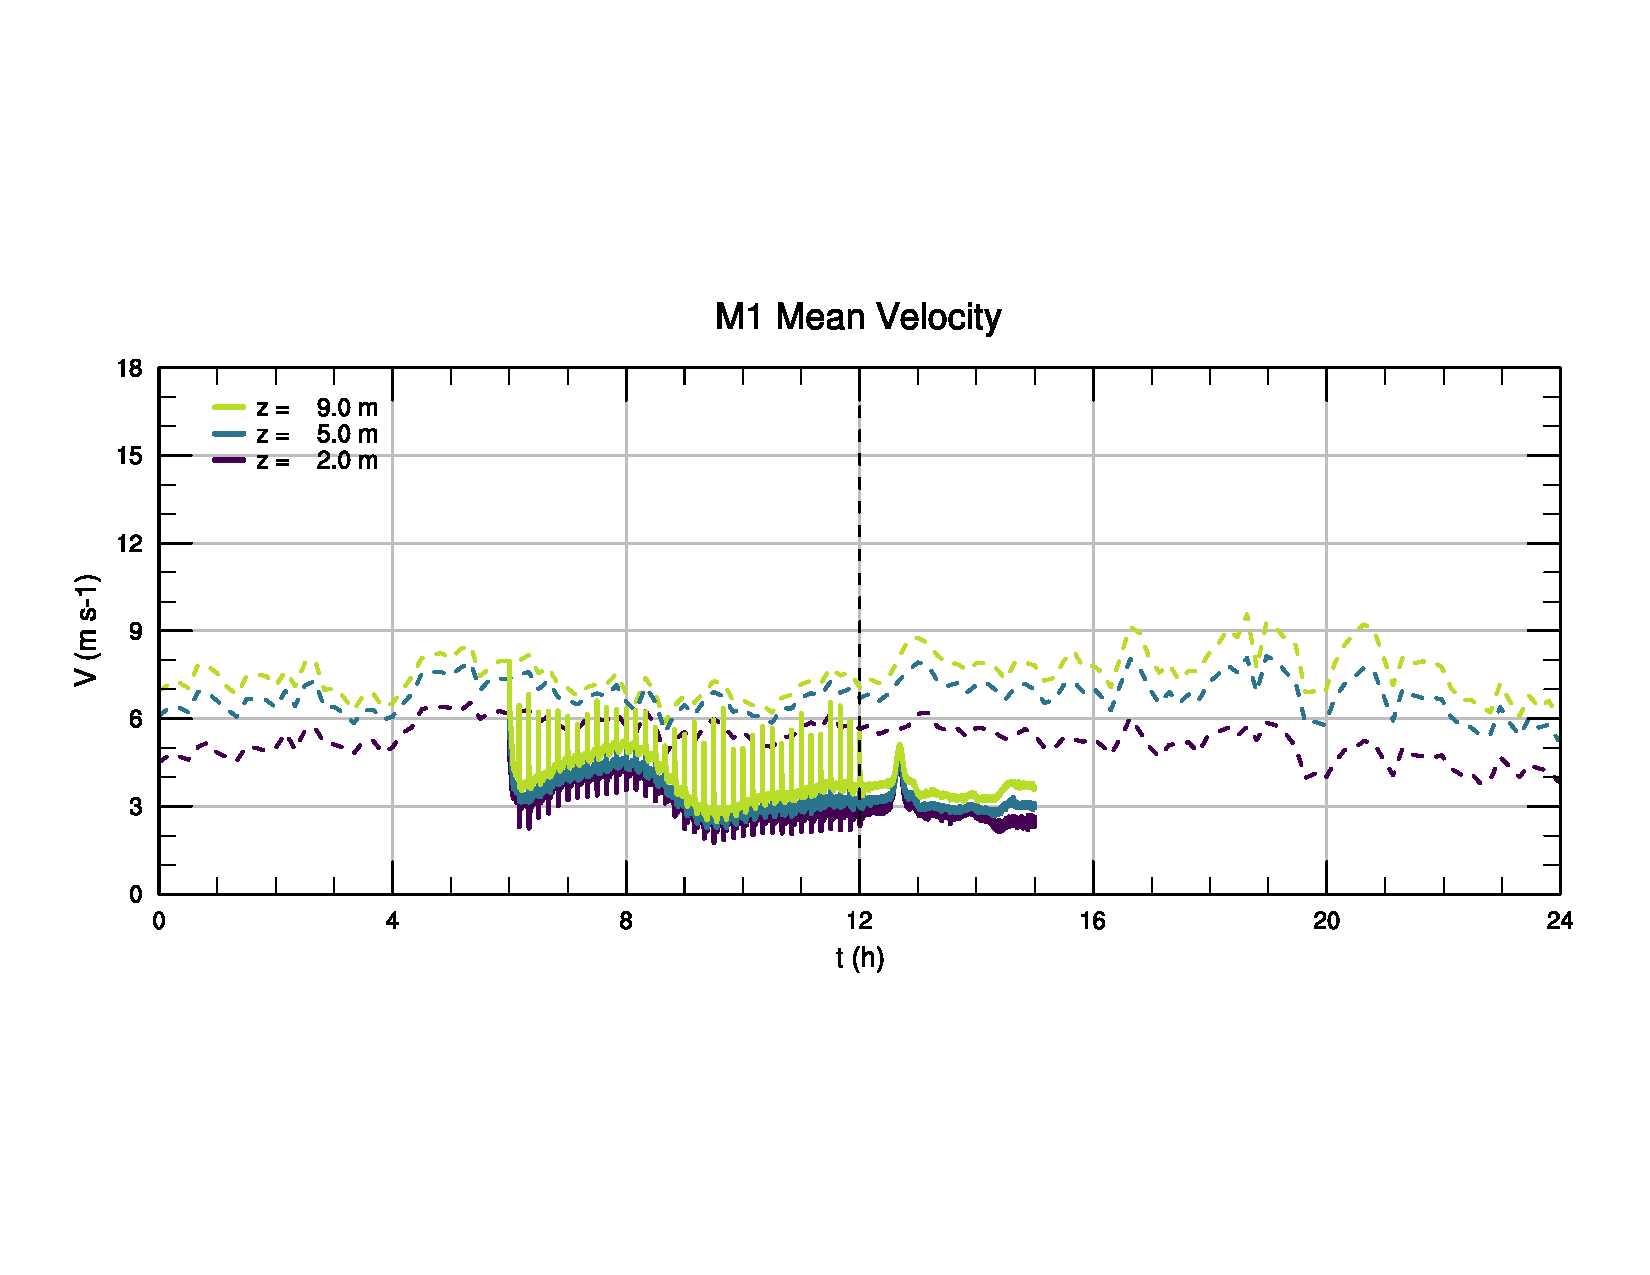
\includegraphics[width=0.87\linewidth,page=1,trim={9mm 57mm 10mm 60mm},clip]{Imagenes/06/bol/ts_interpol_compare.pdf}\\%
	\includegraphics[width=0.87\linewidth,page=1,trim={12mm 52mm 10mm 60mm},clip]{Imagenes/06/bol/ts_interpol_compare_o.pdf}%
	\vspace{-2mm}\caption{Series de tiempo para la rapidez $V$ y dirección $\theta$ del viento en M1.}
	\label{fig:06_bol_ts_m1}
\end{figure}

\begin{figure}[H]
	\centering
	\includegraphics[width=0.87\linewidth,page=2,trim={9mm 57mm 10mm 60mm},clip]{Imagenes/06/bol/ts_interpol_compare.pdf}\\%
	\includegraphics[width=0.87\linewidth,page=2,trim={12mm 52mm 10mm 60mm},clip]{Imagenes/06/bol/ts_interpol_compare_o.pdf}%
	\vspace{-2mm}\caption{Series de tiempo para la rapidez $V$ y dirección $\theta$ del viento en M2.}
	\label{fig:06_bol_ts_m2}
\end{figure}

\begin{figure}[H]
	\centering
	\includegraphics[width=0.87\linewidth,page=3,trim={9mm 57mm 10mm 60mm},clip]{Imagenes/06/bol/ts_interpol_compare.pdf}\\%
	\includegraphics[width=0.87\linewidth,page=3,trim={12mm 52mm 10mm 60mm},clip]{Imagenes/06/bol/ts_interpol_compare_o.pdf}%
	\vspace{-2mm}\caption{Series de tiempo para la rapidez $V$ y dirección $\theta$ del viento en M3.}
	\label{fig:06_bol_ts_m3}
\end{figure}

\begin{figure}[H]
	\centering
	\includegraphics[width=0.87\linewidth,page=4,trim={9mm 57mm 10mm 60mm},clip]{Imagenes/06/bol/ts_interpol_compare.pdf}\\%
	\includegraphics[width=0.87\linewidth,page=4,trim={12mm 52mm 10mm 60mm},clip]{Imagenes/06/bol/ts_interpol_compare_o.pdf}%
	\vspace{-2mm}\caption{Series de tiempo para la rapidez $V$ y dirección $\theta$ del viento en M4.}
	\label{fig:06_bol_ts_m4}
\end{figure}

\begin{figure}[H]
	\centering
	\includegraphics[width=0.87\linewidth,page=5,trim={9mm 57mm 10mm 60mm},clip]{Imagenes/06/bol/ts_interpol_compare.pdf}\\%
	\includegraphics[width=0.87\linewidth,page=5,trim={12mm 52mm 10mm 60mm},clip]{Imagenes/06/bol/ts_interpol_compare_o.pdf}%
	\vspace{-2mm}\caption{Series de tiempo para la rapidez $V$ y dirección $\theta$ del viento en M5.}
	\label{fig:06_bol_ts_m5}
\end{figure}

\begin{figure}[H]
	\centering
	\includegraphics[width=0.87\linewidth,page=6,trim={9mm 57mm 10mm 60mm},clip]{Imagenes/06/bol/ts_interpol_compare.pdf}\\%
	\includegraphics[width=0.87\linewidth,page=6,trim={12mm 52mm 10mm 60mm},clip]{Imagenes/06/bol/ts_interpol_compare_o.pdf}%
	\vspace{-2mm}\caption{Series de tiempo para la rapidez $V$ y dirección $\theta$ del viento en M6.}
	\label{fig:06_bol_ts_m6}
\end{figure}

\begin{figure}[H]
	\centering
	\includegraphics[width=0.87\linewidth,page=7,trim={9mm 57mm 10mm 60mm},clip]{Imagenes/06/bol/ts_interpol_compare.pdf}\\%
	\includegraphics[width=0.87\linewidth,page=7,trim={12mm 52mm 10mm 60mm},clip]{Imagenes/06/bol/ts_interpol_compare_o.pdf}%
	\vspace{-2mm}\caption{Series de tiempo para la rapidez $V$ y dirección $\theta$ del viento en M7.}
	\label{fig:06_bol_ts_m7}
\end{figure}

\begin{figure}[H]
	\centering
	\includegraphics[width=0.87\linewidth,page=8,trim={9mm 57mm 10mm 60mm},clip]{Imagenes/06/bol/ts_interpol_compare.pdf}\\%
	\includegraphics[width=0.87\linewidth,page=8,trim={12mm 52mm 10mm 60mm},clip]{Imagenes/06/bol/ts_interpol_compare_o.pdf}%
	\vspace{-2mm}\caption{Series de tiempo para la rapidez $V$ y dirección $\theta$ del viento en M8.}
	\label{fig:06_bol_ts_m8}
\end{figure}
\subsubsection{Variables de Segundo Orden}
Los siguientes resultados de segundo orden se muestran con el objetivo de aportar a la literatura existente información relevante para la simulación sobre terreno complejo a alta resolución.

Con respecto a los datos mostrados en la Figura \ref{fig:06_bol_mean_secondorder}, el TKE y el esfuerzo turbulento toman las formas clásicas para una capa superficial. El disparo de los valores de M1 y M4 se deben a tres razones: (i) M4 corresponde a una zona de alta nolinealidad, (ii) existe interacción con el terreno complejo en esos puntos y (iii) los valores para $u_*$  son bajos (ver leyenda de la figura). Para $\Phi_M$, en los primeros niveles de M2 y M3, se obtiene un valor muy cercano a la unidad, siendo consistente con la teoría de Monin-Obukhov, sin embargo luego se desvian tomando un valor de aproximadamente $4$. Los puntos M1-M4 ven alterado su comportamiento de $\Phi_M$ debido a su interacción con el terreno complejo adquiriendo valores mayores a $10$.

\begin{figure}[H]
	\begin{minipage}{0.33\linewidth}
		\centering \hspace{1cm}(a)
	\end{minipage}%
	\begin{minipage}{0.33\linewidth}
		\centering \hspace{0.8cm}(b)
	\end{minipage}%
	\begin{minipage}{0.33\linewidth}
		\centering \hspace{0.5cm}(c)
	\end{minipage}%
	\vspace{-4mm}
	\begin{center}
		\includegraphics[height=0.5\linewidth,page=1,trim={6mm 5mm 3mm 0mm},clip]{Imagenes/06/bol/second_order_mean}%
		\includegraphics[height=0.5\linewidth,page=2,trim={12mm 5mm 3mm 0mm},clip]{Imagenes/06/bol/second_order_mean}%
		\includegraphics[height=0.5\linewidth,page=3,trim={12mm 5mm 3mm 0mm},clip]{Imagenes/06/bol/second_order_mean}%
	\end{center}
	\vspace{-5mm}
	\caption{Variables adimensionalizadas de segundo orden para M1-M4 promediadas entre las 12:00 y las 15:00. (a) Energía cinética turbulenta de submalla, (b) Gradiente de velocidad, (c) Esfuerzo turbulento. }
	\label{fig:06_bol_mean_secondorder}
\end{figure}
\newpage
Análogo al caso I, la Figura \ref{fig:06_bol_spectrum} muestra el espectro bidimensional para los primeros 5 niveles verticales del modelo en su dominio mas interior. Se pueden notar una serie de diferencias en contraste con lo obtenido en terreno plano: (i) Existe una mayor cantidad de energía turbulenta asociada a las escalas grandes, hecho que se puede ver en las series de tiempo, (ii) El rango inercial de la cascada de energía cae de manera distinta a la ley de los -5/3, evidenciando la interacción con el terreno complejo y (iii) La disipación en la microescala actúa de manera distinta.

\begin{figure}[H]
	\centering
	\includegraphics[width=1.0\linewidth,page=1,trim={3mm 5mm 3mm 3mm},clip]{Imagenes/06/bol/spectra}%
	\caption{Espectros de energía para la componente horizontal del viento a distintos niveles verticales en el dominio d08 caso Bolund.}
	\label{fig:06_bol_spectrum}
\end{figure}
\subsubsection{Estadísticos}
Las Figuras \ref{fig:06_corr_bol1} y \ref{fig:06_corr_bol2} muestran los gráficos de dispersión entre la rapidez horizontal simulada y real para cada mástil con su correspondiente coeficiente de correlación. Como se pudo observar en las series de tiempo, el modelo fue incapaz de representar correctamente lo medido y por lo tanto se puede ver que todos los coeficientes de correlación con considerablemente bajos.

Finalmente, se obtiene un valor de $2.6724$ [m/s] para el MAE, y $2.9538$ [m/s] para el RMSE.
\newpage
\vspace*{\fill}
\begin{figure}[H]
	\centering
	\includegraphics[width=0.5\linewidth,page=1,trim={0cm 0cm 0cm 0cm},clip]{Imagenes/06/bol/corr}%
	\includegraphics[width=0.5\linewidth,page=2,trim={0cm 0cm 0cm 0cm},clip]{Imagenes/06/bol/corr}%
	
	\includegraphics[width=0.5\linewidth,page=3,trim={0cm 0cm 0cm 0cm},clip]{Imagenes/06/bol/corr}%
	\includegraphics[width=0.5\linewidth,page=4,trim={0cm 0cm 0cm 0cm},clip]{Imagenes/06/bol/corr}%
	\caption{Gráfico de dispersión para las velocidades a distintas alturas en los mástiles M1-M4 en Bolund.}
	\label{fig:06_corr_bol1}
\end{figure}
\vspace*{\fill}
\newpage
\vspace*{\fill}
\begin{figure}[H]
	\centering
	\includegraphics[width=0.5\linewidth,page=5,trim={0cm 0cm 0cm 0cm},clip]{Imagenes/06/bol/corr}%
	\includegraphics[width=0.5\linewidth,page=6,trim={0cm 0cm 0cm 0cm},clip]{Imagenes/06/bol/corr}%
	
	\includegraphics[width=0.5\linewidth,page=7,trim={0cm 0cm 0cm 0cm},clip]{Imagenes/06/bol/corr}%
	\includegraphics[width=0.5\linewidth,page=8,trim={0cm 0cm 0cm 0cm},clip]{Imagenes/06/bol/corr}%
	\caption{Gráfico de dispersión para las velocidades a distintas alturas en los mástiles M5-M8 en Bolund.}
	\label{fig:06_corr_bol2}
\end{figure}
\vspace*{\fill}
\newpage





























\section{Caso II: Bolund con Asimilación Multipunto}
\subsubsection{Estratificación y Largo de Capa Límite}
Si bien la asimilación de datos no cambia la neutralidad de la capa límite, ni la decisión tomada para el largo $\delta$ de altura de ABL, si logró modificar considerablemente la distribución de las lineas horarias  de la Figura \ref{fig:06_bol_da_pbl} con respecto al gráfico sin DA. Esto nos da una primera aproximación a la influencia que tuvo el DA sobre el dominio, la capacidad de desplazar los perfiles de temperatura potencial virtual.

\begin{figure}[H]
	\begin{minipage}{0.5\linewidth}
		\centering{\hspace{0.9cm}(a)}
	\end{minipage}%
	\begin{minipage}{0.5\linewidth}
		\centering{\hspace{0.6cm}(b)}
	\end{minipage}%
	
	\begin{minipage}{0.5\linewidth}
		\centering
		\includegraphics[width=0.9\linewidth,trim={0cm 5mm 0cm 0mm},clip]{Imagenes/06/bol_da/mean_pbl}%
	\end{minipage}%
	\begin{minipage}{0.5\linewidth}
		\centering
		\includegraphics[width=0.9\linewidth,trim={0cm 5mm 0cm 0cm},clip]{Imagenes/06/bol_da/mean_profile}%
	\end{minipage}%
	
	\caption{Ciclo horario del perfil de temperatura potencial virtual promedio de los 8 mástiles (con DA). (a) Resultados cada 10 minutos del perfil de $\theta$. (b) Detalle del perfil dentro de la capa límite atmosférica con resultados cada 15 minutos ($\delta\approx300$ [m]).}
	\label{fig:06_bol_da_pbl}
\end{figure}
\subsubsection{Estructura del Campo de Velocidades}
El dominio muestra dos grandes diferencias con respecto a las lineas de flujo en la Figura \ref{fig:06_bol_da_st}. Primero, hay un déficit notable en la magnitud de la velocidad para todo el dominio y segundo, el vórtice generado por la separación aguas abajo del flujo adquiere otra estructura. Notar como en el primer cuadro se aprecia la influencia del último proceso de asimilación de datos correspondiente a las 12:00.

\begin{figure}[H]
	\begin{minipage}{0.5\linewidth}
		\centering
		\hspace{1cm}(a)
	\end{minipage}%
	\begin{minipage}{0.5\linewidth}
		\centering
		\hspace{-1cm}(b)
	\end{minipage}%
	
	\begin{minipage}{0.5\linewidth}
		\centering
		\includegraphics[height=0.70\linewidth,page=73,trim={12mm 31mm 50mm 20mm},clip]{Imagenes/06/bol_da/eta1}%
	\end{minipage}%
	\begin{minipage}{0.5\linewidth}
		\centering
		\includegraphics[height=0.70\linewidth,page=85,trim={37mm 31mm 20mm 20mm},clip]{Imagenes/06/bol_da/eta1}%
	\end{minipage}%
	\vspace{1mm}
	
	\begin{minipage}{0.5\linewidth}
		\centering
		\hspace{1cm}(c)
	\end{minipage}%
	\begin{minipage}{0.5\linewidth}
		\centering
		\hspace{-1cm}(d)
	\end{minipage}%
	
	\begin{minipage}{0.5\linewidth}
		\centering
		\includegraphics[height=0.73\linewidth,page=97,trim={12mm 23mm 50mm 20mm},clip]{Imagenes/06/bol_da/eta1}%
	\end{minipage}%
	\begin{minipage}{0.5\linewidth}
		\centering
		\includegraphics[height=0.73\linewidth,page=109,trim={37mm 23mm 20mm 20mm},clip]{Imagenes/06/bol_da/eta1}%
	\end{minipage}%
	\caption{Lineas de flujo para la solución numérica en Bolund (con DA) en el primer nivel ($z_1 = 1.12$ [m]) en las horas (a) 12:00, (b) 13:00, (c) 14:00, (d) 15:00.}
	\label{fig:06_bol_da_st}
\end{figure}
En la Figura \ref{fig:06_bol_da_cross} se puede notar de manera mas detallada la disminución global de velocidad en la sección M1-M4. La burbuja de separación disminuyó su largo a un valor de aproximadamente 25 [m]
\subsubsection{Comparación Ciega}
En la Figura \ref{fig:06_bol_da_referencia} se pueden ver los nuevos perfiles referenciales que se usan para el cálculo de las variables adimensionales de comparación. Acá se puede notar que para el flujo no pertubado, la rapidez horizontal disminuyó, en promedio, unos 3 [m/s] en comparación a su contraparte sin DA. La intensidad turbulenta se mantuvo, a grandes rasgos, idéntica al experimento anterior.
\newpage
\vspace*{\fill}
\begin{figure}[H]
	\centering
	\includegraphics[width=0.90\linewidth,trim={0mm 202.0mm 111mm 106mm},clip]{Imagenes/06/bol_da/1200rot}\\%
	\includegraphics[width=0.90\linewidth,trim={0mm 202.0mm 111mm 106mm},clip]{Imagenes/06/bol_da/1300rot}\\%
	\includegraphics[width=0.90\linewidth,trim={0mm 202.0mm 111mm 106mm},clip]{Imagenes/06/bol_da/1400rot}\\%
	\includegraphics[width=0.90\linewidth,trim={0mm 180.0mm 111mm 106mm},clip]{Imagenes/06/bol_da/1500rot}%
	\caption{Contornos de rapidez del viento para la sección de corte a 240$^\circ$ en Bolund (con DA). Se muestran los resultados para las 12:00, 13:00, 14:00 y 15:00 horas. Escala 1:1.}
	\label{fig:06_bol_da_cross}
\end{figure}
\vspace*{\fill}
\newpage

\begin{figure}[H]
	\begin{minipage}{0.5\linewidth}
		\centering{\hspace{0.9cm}(a)}
	\end{minipage}%
	\begin{minipage}{0.5\linewidth}
		\centering{\hspace{0.6cm}(b)}
	\end{minipage}%
	
	\begin{minipage}{0.5\linewidth}
		\centering
		\includegraphics[width=0.7\linewidth,trim={4.5cm 12mm 4.3cm 20mm},clip]{Imagenes/06/bol_da/V_referencia}%
	\end{minipage}%
	\begin{minipage}{0.5\linewidth}
		\centering
		\includegraphics[width=0.7\linewidth,trim={4.5cm 12mm 4.3cm 20mm},clip]{Imagenes/06/bol_da/tke_referencia}%
	\end{minipage}%
	
	\caption{Perfiles promedio referenciales (Bolund con DA) en el flujo no perturbado para: (a) Rapidez del viento (en línea punteada se presenta la condición de contorno presentada por Bechmann et. al., 2011) (b) Intensidad de energía cinética turbulenta (sgs).}
	\label{fig:06_bol_da_referencia}
\end{figure}

Exceptuando el valor correspondiente a las 12:00 (influencia de DA), la distribución de \emph{speedup} mostrada en la Figura \ref{fig:06_bol_da_speedup} no presenta grandes cambios con respecto al caso sin DA. Los valores para todos los $\Delta S$ son inferiores y se puede ver cuantitativamente como disminuyó el largo de la burbuja de separación. La separación que debiese ocurrir cerca de M2 siguió sin manifestarse.

El incremento de la energía cinética turbulenta mostrado en la Figura \ref{fig:06_bol_da_tke} expone un hecho importante para el proceso de asimilación de datos: el TKE a lo largo de todo el dominio se reinicia cada vez que se asimila. Esto explica que el $\Delta k$ sea idénticamente 0 para toda la sección a las 12:00. 

Si bien, gran parte de la información necesaria para ejecutar correctamente el modelo se traspasa a través del archivo en el cual se asimila, la energía cinética turbulenta demorará algún tiempo característico en volver a generarse de manera adecuada, y por lo tanto, es muy probable que la manera cíclica en la que se estuvo asimilando datos para estos casos haya perjudicado la eficacia del tiempo de \emph{spinup}.
\newpage
Con respecto a los valores para el resto de las horas, hubo un aumento considerable para el $\Delta k$ en todos los niveles para el punto cercano a M2 debido probablemente al transiente que generó el proceso de asimilación. En las cercanías de M4, nuevamente no se pudo rescatar todo el aumento deseado.
\vspace*{\fill}
\begin{figure}[H]
	\centering
	\includegraphics[width=0.95\linewidth,trim={12mm 84mm 10mm 74mm},page=1,clip]{Imagenes/06/bol_da/speedup}\\%
	\includegraphics[width=0.95\linewidth,trim={12mm 84mm 10mm 74mm},page=13,clip]{Imagenes/06/bol_da/speedup}\\%
	\includegraphics[width=0.95\linewidth,trim={12mm 84mm 10mm 74mm},page=25,clip]{Imagenes/06/bol_da/speedup}\\%
	\includegraphics[width=0.95\linewidth,trim={12mm 84mm 10mm 74mm},page=37,clip]{Imagenes/06/bol_da/speedup}\\%
	\includegraphics[width=0.95\linewidth,trim={-11mm 193mm 115mm 112mm},clip]{Imagenes/06/bol_da/cross_height}\\%
	\caption{Speedup en los primeros 3 niveles del modelo ($1.1$ [m] azul; $3.4$ [m] verde; $5.6$ [m] amarillo) para la sección de corte a 240$^\circ$ en Bolund (con DA). Se muestran los resultados para las 12:00, 13:00, 14:00 y 15:00 horas.}
	\label{fig:06_bol_da_speedup}
\end{figure}
\vspace*{\fill}
\newpage
\vspace*{\fill}
\begin{figure}[H]
	\centering
	\includegraphics[width=0.90\linewidth,trim={12mm 84mm 10mm 74mm},page=1,clip]{Imagenes/06/bol_da/delta_tke}\\%
	\includegraphics[width=0.90\linewidth,trim={12mm 84mm 10mm 74mm},page=13,clip]{Imagenes/06/bol_da/delta_tke}\\%
	\includegraphics[width=0.90\linewidth,trim={12mm 84mm 10mm 74mm},page=25,clip]{Imagenes/06/bol_da/delta_tke}\\%
	\includegraphics[width=0.90\linewidth,trim={12mm 84mm 10mm 74mm},page=37,clip]{Imagenes/06/bol_da/delta_tke}\\%
	\includegraphics[width=0.90\linewidth,trim={-13.3mm 193mm 115mm 112mm},clip]{Imagenes/06/bol_da/cross_height}\\%
	\caption{Incremento adimnsional de energía cinética turbulenta (sgs) en los primeros 3 niveles del modelo ($1.1$ [m] azul; $3.4$ [m] verde; $5.6$ [m] amarillo) para la sección de corte a 240$^\circ$ en Bolund (con DA). Se muestran los resultados para las 12:00, 13:00, 14:00 y 15:00 horas.}
	\label{fig:06_bol_da_tke}
\end{figure}
\vspace*{\fill}
\newpage
Con respecto a los perfiles en los mástiles mostrados en la Figura \ref{fig:06_bol_da_mast_tke_speedup}: M1 disminuye su \emph{speedup} y aumenta considerablemente su $\Delta k$, alejándose de los datos medidos. M2 y M3 mantienen su comportamiento, con la diferencia de que ahora en M2 hay mas TKE. Esta diferencia en el TKE para M1 y M2, está relacionada con el incremento local de $k$ en las cercanías de esos puntos. M4 mantiene a grandes rasgos lo simulado anteriormente, pero se intensifica el déficit de \emph{speedup} dentro de la burbuja de separación. De manera general, todos los valores están lejanos de los medidos.
\vspace*{\fill}
\begin{figure}[H]
	\begin{minipage}{0.5\linewidth}
		\centering
		\hspace{7mm}(a)\end{minipage}%
	\begin{minipage}{0.5\linewidth}
		\centering
		\hspace{-5mm}(b)\end{minipage}%
	
	\centering
	\includegraphics[height=0.75\linewidth,page=1,trim={28mm 10mm 25mm 23mm},clip]{Imagenes/06/bol_da/V_masts}%
	\includegraphics[height=0.75\linewidth,page=1,trim={30mm 10mm 17mm 20mm},clip]{Imagenes/06/bol_da/k_masts}%
	\vspace{-2mm}\caption{Perfil vertical de (a) \emph{speedup} y (b) variación adimensional de energía cinética turbulenta para M1 (azul), M2 (naranja), M3 (verde) y M4 (rojo) para el caso con DA.}
	\label{fig:06_bol_da_mast_tke_speedup}
\end{figure}
\vspace*{\fill}
\newpage
\subsubsection{Comparación con Series de Tiempo}
A continuación se muestran los resultados para las series de tiempo en la Figuras \ref{fig:06_bol_da_ts_m1}-\ref{fig:06_bol_da_ts_m8}. Se puede ver que los resultados para todos los mástiles empeoraron: los déficit se acentuaron e incluso la dirección se modificó (ver M7). Por otro lado, se puede ver que se rescatan tendecias de las mediciones, como por ejemplo la pequeña ráfaga que ocurre a cerca de las 13:00 y la aceleración leve que ocurre después de esto. El mástil que mejor se comporta al DA es extrañamente M4 (el mas no lineal) encontrándose alta concordancia entre lo simulado y lo real. Los mástiles que antes presentaban cierta intensidad turbulenta ahora la muestran de manera mas fuerte, mostrando cierta relación entre el DA y la turbulencia resuelta.

En general, el proceso de asimilación de datos no fue exitoso. Las discrepancias que se pretendían corregir sólo se acentuaron y las mejorar que se pudieron hallar son demasiado locales como para hacer una regla general. Esto demuestra la complejidad que induce el terreno complejo en el comportamiento del viento y el cuidado especial que se debe tener para simular un caso como este que, a grandes rasgos, sigue siendo sencillo.
\newpage
\begin{figure}[H]
	\centering
	\includegraphics[width=0.87\linewidth,page=1,trim={9mm 57mm 10mm 60mm},clip]{Imagenes/06/bol_da/ts_interpol_compare.pdf}\\%
	\includegraphics[width=0.87\linewidth,page=1,trim={12mm 52mm 10mm 60mm},clip]{Imagenes/06/bol_da/ts_interpol_compare_o.pdf}%
	\vspace{-2mm}\caption{Series de tiempo para la rapidez $V$ y dirección $\theta$ del viento en M1 con DA.}
	\label{fig:06_bol_da_ts_m1}
\end{figure}

\begin{figure}[H]
	\centering
	\includegraphics[width=0.87\linewidth,page=2,trim={9mm 57mm 10mm 60mm},clip]{Imagenes/06/bol_da/ts_interpol_compare.pdf}\\%
	\includegraphics[width=0.87\linewidth,page=2,trim={12mm 52mm 10mm 60mm},clip]{Imagenes/06/bol_da/ts_interpol_compare_o.pdf}%
	\vspace{-2mm}\caption{Series de tiempo para la rapidez $V$ y dirección $\theta$ del viento en M2 con DA.}
	\label{fig:06_bol_da_ts_m2}
\end{figure}

\begin{figure}[H]
	\centering
	\includegraphics[width=0.87\linewidth,page=3,trim={9mm 57mm 10mm 60mm},clip]{Imagenes/06/bol_da/ts_interpol_compare.pdf}\\%
	\includegraphics[width=0.87\linewidth,page=3,trim={12mm 52mm 10mm 60mm},clip]{Imagenes/06/bol_da/ts_interpol_compare_o.pdf}%
	\vspace{-2mm}\caption{Series de tiempo para la rapidez $V$ y dirección $\theta$ del viento en M3 con DA.}
	\label{fig:06_bol_da_ts_m3}
\end{figure}

\begin{figure}[H]
	\centering
	\includegraphics[width=0.87\linewidth,page=4,trim={9mm 57mm 10mm 60mm},clip]{Imagenes/06/bol_da/ts_interpol_compare.pdf}\\%
	\includegraphics[width=0.87\linewidth,page=4,trim={12mm 52mm 10mm 60mm},clip]{Imagenes/06/bol_da/ts_interpol_compare_o.pdf}%
	\vspace{-2mm}\caption{Series de tiempo para la rapidez $V$ y dirección $\theta$ del viento en M4 con DA.}
	\label{fig:06_bol_da_ts_m4}
\end{figure}

\begin{figure}[H]
	\centering
	\includegraphics[width=0.87\linewidth,page=5,trim={9mm 57mm 10mm 60mm},clip]{Imagenes/06/bol_da/ts_interpol_compare.pdf}\\%
	\includegraphics[width=0.87\linewidth,page=5,trim={12mm 52mm 10mm 60mm},clip]{Imagenes/06/bol_da/ts_interpol_compare_o.pdf}%
	\vspace{-2mm}\caption{Series de tiempo para la rapidez $V$ y dirección $\theta$ del viento en M5 con DA.}
	\label{fig:06_bol_da_ts_m5}
\end{figure}

\begin{figure}[H]
	\centering
	\includegraphics[width=0.87\linewidth,page=6,trim={9mm 57mm 10mm 60mm},clip]{Imagenes/06/bol_da/ts_interpol_compare.pdf}\\%
	\includegraphics[width=0.87\linewidth,page=6,trim={12mm 52mm 10mm 60mm},clip]{Imagenes/06/bol_da/ts_interpol_compare_o.pdf}%
	\vspace{-2mm}\caption{Series de tiempo para la rapidez $V$ y dirección $\theta$ del viento en M6 con DA.}
	\label{fig:06_bol_da_ts_m6}
\end{figure}

\begin{figure}[H]
	\centering
	\includegraphics[width=0.87\linewidth,page=7,trim={9mm 57mm 10mm 60mm},clip]{Imagenes/06/bol_da/ts_interpol_compare.pdf}\\%
	\includegraphics[width=0.87\linewidth,page=7,trim={12mm 52mm 10mm 60mm},clip]{Imagenes/06/bol_da/ts_interpol_compare_o.pdf}%
	\vspace{-2mm}\caption{Series de tiempo para la rapidez $V$ y dirección $\theta$ del viento en M7 con DA.}
	\label{fig:06_bol_da_ts_m7}
\end{figure}

\begin{figure}[H]
	\centering
	\includegraphics[width=0.87\linewidth,page=8,trim={9mm 57mm 10mm 60mm},clip]{Imagenes/06/bol_da/ts_interpol_compare.pdf}\\%
	\includegraphics[width=0.87\linewidth,page=8,trim={12mm 52mm 10mm 60mm},clip]{Imagenes/06/bol_da/ts_interpol_compare_o.pdf}%
	\vspace{-2mm}\caption{Series de tiempo para la rapidez $V$ y dirección $\theta$ del viento en M8 con DA.}
	\label{fig:06_bol_da_ts_m8}
\end{figure}
\subsubsection{Variables de Segundo Orden}
En la Figura \ref{fig:06_bol_da_mean_secondorder} se muestran las variables de segundo orden para el caso con DA. Se puede ver que la incorporación de los datos hizo disminuir los valores de $u_*$ para todos los mástiles, especialmente en M4 y esto explica el disparo de los valores de $k$ y $\tau_{13}$ adimensionalizados. La curva del gradiente de velocidad para M1 volvió a valores mas relacionados con la neutralidad, mientras que M4 continúa su comportamiento errático por el desprendimiento. De todas formas, el comportamiento de estas variables es según lo esperado.
\begin{figure}[H]
	\begin{minipage}{0.33\linewidth}
		\centering \hspace{1cm}(a)
	\end{minipage}%
	\begin{minipage}{0.33\linewidth}
		\centering \hspace{0.8cm}(b)
	\end{minipage}%
	\begin{minipage}{0.33\linewidth}
		\centering \hspace{0.5cm}(c)
	\end{minipage}%
	\vspace{-4mm}
	\begin{center}
		\includegraphics[height=0.5\linewidth,page=1,trim={6mm 5mm 3mm 0mm},clip]{Imagenes/06/bol_da/second_order_mean}%
		\includegraphics[height=0.5\linewidth,page=2,trim={12mm 5mm 3mm 0mm},clip]{Imagenes/06/bol_da/second_order_mean}%
		\includegraphics[height=0.5\linewidth,page=3,trim={12mm 5mm 3mm 0mm},clip]{Imagenes/06/bol_da/second_order_mean}%
	\end{center}
	\vspace{-5mm}
	\caption{Variables adimensionalizadas de segundo orden para M1-M4 con DA, promediadas entre las 12:00 y las 15:00. (a) Energía cinética turbulenta de submalla, (b) Gradiente de velocidad, (c) Esfuerzo turbulento. }
	\label{fig:06_bol_da_mean_secondorder}
\end{figure}
Con respecto al espectro de velocidades en la Figura \ref{fig:06_bol_da_spectrum}, sorpresivamente ahora no se muestra el \emph{backscatter} que presentó el caso de terreno plano, probablemente porque el forzamiento debido a la interacción con el terreno complejo sea dominante sobre el forzamiento que causa la asimilación de datos, sin embargos si existen comportamientos ruidosos luego del número de onda de \emph{cutoff}. Las pendientes para la zona inercial se ven modificadas: el primer nivel tiene una un poco mas empinada (explicada por el ingreso de energía que se da a esa escala), y los niveles superiores tienen un comportamiento con una pendiente menor que -5/3, siendo quizás mas difusivos.
\newpage
\begin{figure}[H]
	\centering
	\includegraphics[width=1.0\linewidth,page=1,trim={3mm 5mm 3mm 3mm},clip]{Imagenes/06/bol_da/spectra}%
	\caption{Espectros de energía para la componente horizontal del viento a distintos niveles verticales en el dominio d08 caso Bolund con DA.}
	\label{fig:06_bol_da_spectrum}
\end{figure}
\subsubsection{Estadísticos}
Con respecto a los gráficos de dispersión presentados en las Figuras \ref{fig:06_corr_bol1_da} y \ref{fig:06_corr_bol2_da}, si bien existen algunas mejoras específicas, como por ejemplo M1, en general los coeficientes de correlación empeoraron.  

Ahora, es notable de cierta manera que, la asimilación de datos multipunto a nivel de superficie y a esta escala, logre alterar tan fuertemente el comportamiento del campo de velocidades. Lo esperado era tener desviaciones tenues, tal como se tuvo para Høvsøre. Esto manifiesta el cuidado que se debe tener al incorporar datos y que esta área aún es fértil para investigar.

El resumen del resto de los estadísticos se puede ver en la Tabla \ref{tab:06_bol_mae_rmse}. La pérdida de precisión da como resultado una variación de aproximadamente -60\% para las métricas seleccionadas.

\begin{table}[h!]
	\caption{Comparación de métricas para el caso II Bolund.}
	\label{tab:06_bol_mae_rmse}
	\centering%\footnotesize
	\begin{tabular}{lcc}
		\toprule
		& Sin DA & Con DA \\
		\midrule
		MAE & 2.6724 m/s & 4.3562 m/s \\
		RMSE & 2.9538 m/s& 4.90071 m/s\\
		$\Delta{RMSE}$&  -- & $-65.91\%$ \\
		$\Delta{MAE}$ &  -- & $-63.01\%$ \\
		\bottomrule
	\end{tabular}
\end{table}
\newpage
\vspace*{\fill}
\begin{figure}[H]
	\centering
	\includegraphics[width=0.5\linewidth,page=1,trim={0cm 0cm 0cm 0cm},clip]{Imagenes/06/bol_da/corr}%
	\includegraphics[width=0.5\linewidth,page=2,trim={0cm 0cm 0cm 0cm},clip]{Imagenes/06/bol_da/corr}%
	
	\includegraphics[width=0.5\linewidth,page=3,trim={0cm 0cm 0cm 0cm},clip]{Imagenes/06/bol_da/corr}%
	\includegraphics[width=0.5\linewidth,page=4,trim={0cm 0cm 0cm 0cm},clip]{Imagenes/06/bol_da/corr}%
	\caption{Gráfico de dispersión para las velocidades a distintas alturas en los mástiles M1-M4 en Bolund (con DA).}
	\label{fig:06_corr_bol1_da}
\end{figure}
\vspace*{\fill}
\newpage
\vspace*{\fill}
\begin{figure}[H]
	\centering
	\includegraphics[width=0.5\linewidth,page=5,trim={0cm 0cm 0cm 0cm},clip]{Imagenes/06/bol_da/corr}%
	\includegraphics[width=0.5\linewidth,page=6,trim={0cm 0cm 0cm 0cm},clip]{Imagenes/06/bol_da/corr}%
	
	\includegraphics[width=0.5\linewidth,page=7,trim={0cm 0cm 0cm 0cm},clip]{Imagenes/06/bol_da/corr}%
	\includegraphics[width=0.5\linewidth,page=8,trim={0cm 0cm 0cm 0cm},clip]{Imagenes/06/bol_da/corr}%
	\caption{Gráfico de dispersión para las velocidades a distintas alturas en los mástiles M5-M8 en Bolund (con DA).}
	\label{fig:06_corr_bol2_da}
\end{figure}
\vspace*{\fill}

